% TEMPLATE for Usenix papers, specifically to meet requirements of
%  USENIX '05
% originally a template for producing IEEE-format articles using LaTeX.
%   written by Matthew Ward, CS Department, Worcester Polytechnic Institute.
% adapted by David Beazley for his excellent SWIG paper in Proceedings,
%   Tcl 96
% turned into a smartass generic template by De Clarke, with thanks to
%   both the above pioneers
% use at your own risk.  Complaints to /dev/null.
% make it two column with no page numbering, default is 10 point

% Munged by Fred Douglis <douglis@research.att.com> 10/97 to separate
% the .sty file from the LaTeX source template, so that people can
% more easily include the .sty file into an existing document.  Also
% changed to more closely follow the style guidelines as represented
% by the Word sample file. 

% Note that since 2010, USENIX does not require endnotes. If you want
% foot of page notes, don't include the endnotes package in the 
% usepackage command, below.

% This version uses the latex2e styles, not the very ancient 2.09 stuff.
\documentclass[letterpaper,twocolumn,10pt]{article}
\usepackage{usenix,epsfig}
\usepackage{color}

\usepackage{graphicx, subfigure}
\usepackage{url}

\def\todo#1{{\bf \textcolor{red}{TODO:~#1}}}
\def\question#1{{\bf \textcolor{purple}{Question:~#1}}}
\def\comment#1{{\bf \textcolor{blue}{~#1}}}
\def\etal{et\ al.\ }

\begin{document}

%don't want date printed
\date{}

%make title bold and 14 pt font (Latex default is non-bold, 16 pt)
\title{\Large \bf TrustFA: TrustZone-Assisted Facial Authentication on Smartphone}

%for single author (just remove % characters)
\author{
{\rm Dongli Zhang}\\
Stony Brook University
\and
{\rm Radu Sion}\\
Stony Brook University
% copy the following lines to add more authors
% \and
% {\rm Name}\\
%Name Institution
} % end author

\maketitle

% Use the following at camera-ready time to suppress page numbers.
% Comment it out when you first submit the paper for review.
\thispagestyle{empty}


\subsection*{Abstract}

Nowadays, many applications, such as Facebook, Dropbox and mobile banking,
allow users to login and use the remote services via smartphones. Because of
the limitations of credential-based authentication, biometric authentication is
becoming popular. Facial authentication is one of the popular biometric
authentication techniques and it consists of three phases: first, the photo is
captured by hardware camera; second, the smartphone application retrieves the
photo from hardware camera via OS; third, the smartphone application
authenticates the user by sending the photo (or its extracted features) to
remote services.  To achieve the trusted facial authentication, all three
phases should be secured.  In this paper, we propose TrustFA, a
TrustZone-assisted solution to secure all three phases in facial authentication
on smartphone.  We leverage the ARM TrustZone technique to capture the photo
and collect the accelerometer data in TrustZone secure world.  As all of the
secure world memory, peripherals and interrupts are isolated from normal world
legacy OS, attackers even with root privilege in legacy OS would not be able to
break the authentication. Within our knowledge, this is the first effort that
all of three phases in facial authentication are secured. Compared to prior
works, the threat model regarding smartphone facial authentication assumed in
this paper is the most strongest.  Since the prototyping is still in progress,
we envision the implementation of TrustFA on Freescale i.MX53 Quick Start Board
(QSB).


%However, 2D facial authentication still has two issues. First, 2D media attack
%makes the 2D facial authentication untrusted. The attacker could just put a
%photo in front of the camera to cheat the authentication program.  Second, the
%large TCB of legacy OS makes the smartphone vulnerable to malwares.  The
%untrusted legacy OS would tamper the photo/video captured by the camera (e.g.,
%virtual camera attack). 

\section{Introduction}
\label{sec:introduction}

Recent years have experienced explosive growth of smartphone sales and
smartphones become pervasive. By March 2013, Google has activated more than 750M
Android-based devices \cite{Google-ARM}.  Smartphones are no longer basic
devices for making phone calls and receiving text messages, but powerful
platforms with comparable functionalities to commodity PCs.  Mobile applications
provide users the functionality to access the data maintained by remote services
such as Dropbox, Facebook, and online banking. The credential-based
authentication requires the users to provide the password (PIN), which can be
figured out by the attacker via social engineering attack. The longer the length of
password, the more time consumed by the user to manually input the password.
Recently, Shukla \etal \cite{Hand-Secret} introduce a side-channel attack on
the PIN entry process on a smartphone. The attack is entirely based on the
spatio-temporal dynamics of the hands during typing to decode the typed text. It
is demonstrated that the attack breaks an average of over 85\% of the PINs in
ten attempts on a dataset of 200 videos of the PIN entry process.

Compared to the credential-based authentication, biometric authentication is
widely considered more secure. Unlike credential-based authentication
which depends on "the knowledge of user", biometric authentication relies on "the
identity of user" which is very difficult for attackers to forge.

Facial authentication is one of the popular biometric authentication techniques.
 As shown in Figure \ref{fig:dataflow}, the data flow of
facial authentication consists of three phases. First, the photo is captured by
hardware camera on smartphone.  Second, the smartphone application obtains
the photo via the OS.  Finally, the smartphone application (processes the photo
and) sends the photo (or its extracted features) to the remote server. To achieve a trusted facial
authentication, all of three phases, which are vulnerable to attacks,  should be
secured. Even if the device has a front camera, it is rarely used in practice because of
its own limitations.

\begin{figure}[htb]
	\centering
	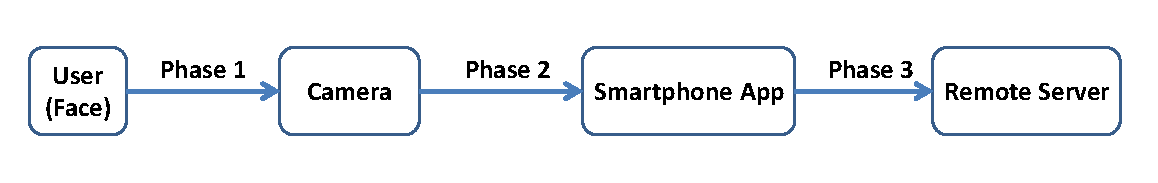
\includegraphics[width=1.0\columnwidth]{figures/dataflow.eps}
	\caption{Facial Authentication Data Flow}
	\label{fig:dataflow}
\end{figure}

\noindent
{\bf Phase 1~}
The first phase is vulnerable to 2D media attack. Instead of the real 3D face,
the attacker can easily fool the 2D face recognition by a flat photo of the
user, which is not difficult to download from social networks
\cite{android-attack}.  Although more
sophisticated 3D facial authentication techniques have been proposed to achieve
higher security \cite{Chaua-3D, Blanz-3D},  the image processing always consumes
a lot of time and the ease of use is also compromised.  For instance, to
differentiate a real 3D face from a flat photo, the Toshiba Face Recognition
Utility requires users to turn their heads towards four directions according to
a sequence of arrows shown on the screen, and the whole authentication process
takes about 30 seconds.  In this paper, we leverage the solution
proposed by Chen \etal in \cite{Chen-Sensor} to secure the first phase. Besides
the user photo, accelerometer is employed to infer the position and orientation
of the front camera. A small movement of the cellphone is applied to ensure a
real 3D face. Although the proposal of \cite{Chen-Sensor} is more efficient than 3D
facial authentication, it is still vulnerable in the second phase. 

\noindent
{\bf Phase 2~}
In the second phase, the photo (video) is retrieved by the smartphone application via
the legacy OS. On the smartphone, the large TCB of legacy OS, e.g., Android,
makes it vulnerable to malwares.  The untrusted legacy OS would tamper the
photo/video captured by the camera (e.g., virtual camera attack), or replace the
captured photo/video with pre-captured ones. Although Chen \etal
\cite{Chen-Sensor} propose Motion Vector Correlation, that is, to extract the
non-intentional shakes of user from both the video and accelerometer, and to
verify if they are correlated with each other, they assume the legacy OS is
trusted, that is, the attacker is not able to tamper the collected data at OS
level.  Besides, the computation overhead of Motion Vector Correlation is also
relatively high. To overcome the limitation in \cite{Chen-Sensor}, we leverage the
ARM TrustZone technology to ensure the trust of data from camera/accelerometer.
Both photo and accelerations are collected in TrustZone secure world.  Attackers
even with root privilege in legacy OS would not be able to compromise the
integrity and freshness of the collected data. The performance overhead of
TrustZone world switch is trivial compared to Motion Vector Correlation in
\cite{Chen-Sensor}.

\noindent
{\bf ARM TrustZone~}
TrustZone is a security extension introduced by ARM. The basic idea is to
logically partition the computing platform into two execution domains: the
normal world and the secure world.  To facilitate context switch between the two
worlds, monitor mode is introduced as the only entry point from normal world to
secure world.  Execution in the normal world jumps to the secure world by
explicitly issuing the Secure Monitor Call (SMC) instruction.  The secure world
can access the full range of the physical memory and all hardware peripherals.
On the other hand, some physical memory ranges and hardware peripherals can be
restricted to be only accessed by the secure world. Therefore, these secure
physical memory and hardware peripherals are under full hardware-based
protections from attacks that can potentially compromise the normal world legacy
OS.  Besides, interrupts and DMA are also world-aware.

\noindent
{\bf Phase 3~}
In the third phase, the photo (or features extracted from photos) is sent to the remote service to
authenticate the user. As this phase can be secured by SSL/TLS, we will not
discuss the detail in the paper.

In this paper, we propose TrustFA, a TrustZone-assisted facial authentication
to secure all three phases mentioned above.  The capture of photo, the
collection of accelerations, and the encryption/decryption of related data are
performed in TrustZone secure world.  As all of the secure world memory,
peripherals and interrupts are isolated from normal world legacy OS, attackers
even with root privilege in legacy OS would not be able to break the
authentication.  In summary, we make the following contributions in the paper: 
\begin{itemize}
\item We propose TrustFA, a TrustZone-assisted facial authentication.  Within
our knowledge, this is the first effort that all three phases in facial
authentication are secured. Compared to prior works, especially
\cite{Chen-Sensor}, the threat model regarding smartphone facial authentication
assumed in this paper is the most strongest.

\item As we leverage ARM TrustZone to ensure the trust and freshness of
camera/accelerometer data source, the performance overhead of securing Phase 2 is
only the overhead of TrustZone switch.  The future work only needs to
focus on how to more efficiently prevent 2D media attack.

\item Since the prototyping is still in progress, we envision the implementation of TrustFA on Freescale i.MX53 Quick Start
Board (QSB). We demonstrate the preliminary performance evaluation of TrustZone
world switch. Our vision is also applicable on other ARM development boards.
\end{itemize}

\section{Design}
\label{sec:design}

\subsection{Overview}
\label{sec:design:overview}

The architecture of TrustFA is in Figure \ref{fig:arch}. We assume the
smartphone is running Android OS as the legacy OS. Besides the legacy OS in
TrustZone normal world, a secure kernel is placed in secure world. The secure
kernel can be either a customized Linux kernel or a new tiny kernel developed
from scratch (e.g., xv6 \cite{xv6}).  The device first boots into the secure
kernel in secure world which then boots the legacy OS in normal world. Touch
screen driver, display driver, crypto library and computer vision library (e.g.,
OpenCV) are ported to secure world kernel. A kernel module (tz.ko) is loaded in
normal world for the communication between two worlds.

\begin{figure}[htb]
	\centering
	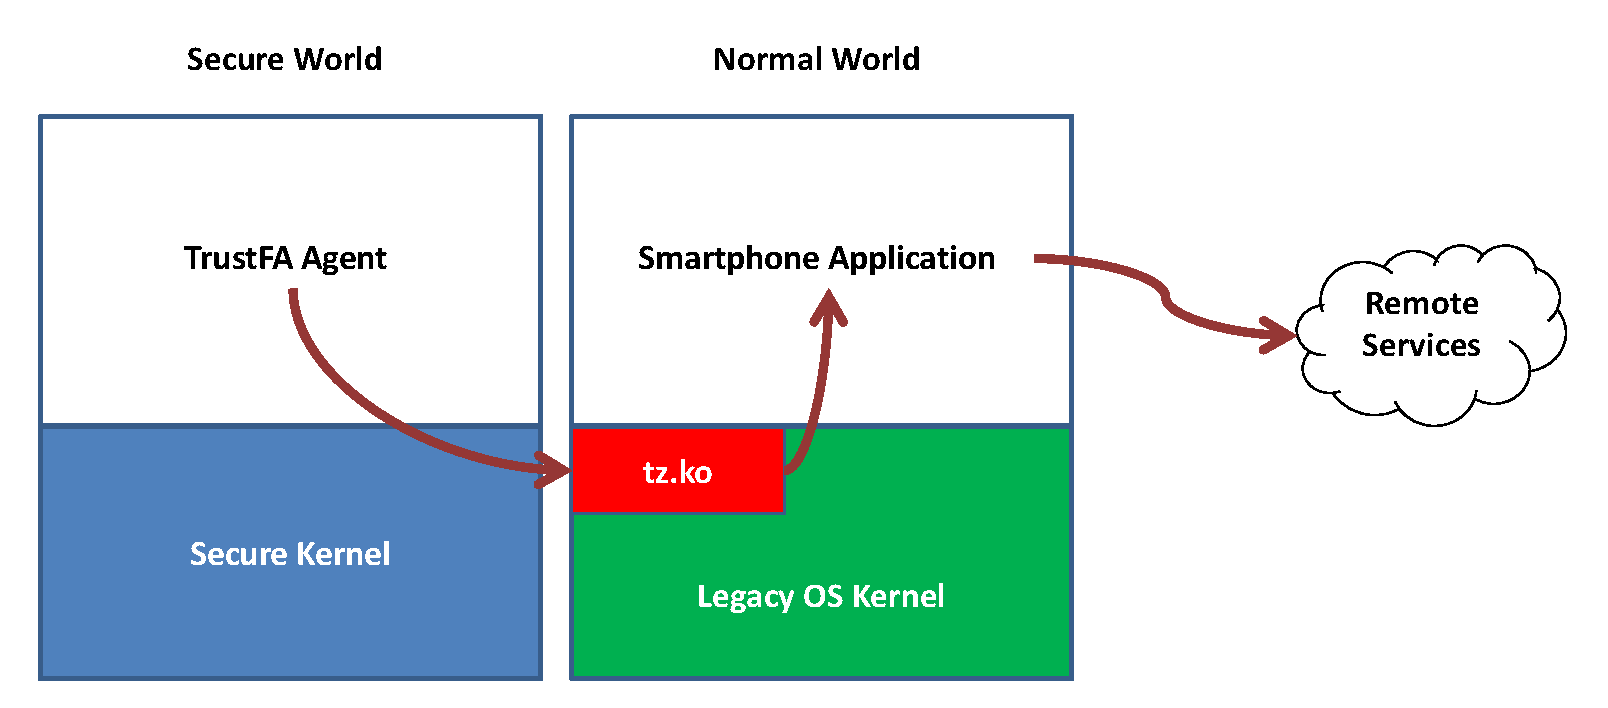
\includegraphics[width=1.0\columnwidth]{figures/arch.eps}
	\caption{TrustFA Architecture}
	\label{fig:arch}
\end{figure}

\begin{figure*}[htb]
	\centering
	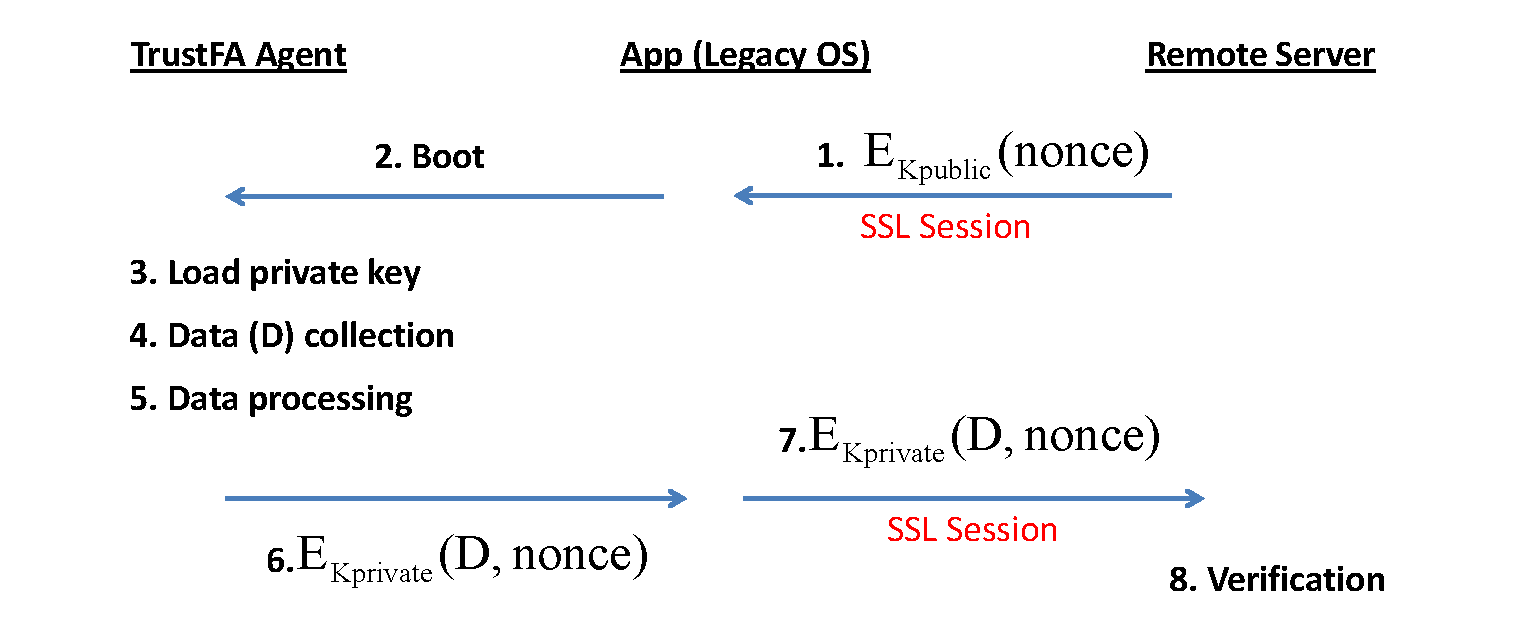
\includegraphics[width=2.0\columnwidth]{figures/authentication.eps}
	\caption{TrustFA Facial Authentication Workflow}
	\label{fig:authentication}
\end{figure*}

\noindent
{\bf Trust Model~}
Our trust model is rooted in the hardware isolation provided by the ARM
TrustZone. The TCB includes secure kernel and TrustFA Agent in secure world. We
assume the legacy OS is untrusted and can be potentially malicious. If the
legacy OS becomes compromised, the TrustZone ensures the integrity and
confidentiality of code and data residing in the secure world. Besides, we
assume the attacker is able to obtain the flat photo and video of user from social
networks to mount the 2D media attack..

Secure boot ensures that only the untampered image can pass the integrity check
of the chip and boot on the device (Section \ref{sec:implementation}).  The
device owns a device key $K_{DEV}$ which is flashed permanently on the one-time
programmable (OTP) fuses. Only secure world has access to fuses to retrieve
$K_{DEV}$. Besides, a key pair ($K_{public}$ and $K_{private}$) is generated.  $K_{public}$ is placed on the remote server provisioning the
service. $K_{private}$ is encrypted with $K_{DEV}$ (as
$E_{K_{DEV}}{(K_{private})}$) and stored on the persistent storage. The secure
kernel retrieves the encrypted $K_{private}$ (as $E_{K_{DEV}}{(K_{private})}$) via
the normal world legacy OS storage driver and decrypt it with $K_{DEV}$ in
secure world. As $K_{DEV}$ is only accessible in secure world, the legacy OS is
not able to obtain $K_{private}$ in normal world. 

\subsection{2D Media Attack}
\label{sec:design:phase1}

To differentiate the 3D face from 2D counterfeits, we leverage the solution in
\cite{Chen-Sensor} to correlate the camera with the accelerometer. As soon as
the authentication starts, the user moves the smartphone horizontally for a
short distance in front of the face from left to right. Once the face area is
greater or equal to 40\% area of the video frame, the smartphone starts sampling
video (from camera) and accelerations (from accelerometer). Once the face area
is smaller than 30\%, the sampling stops.

TrustFA Agent analyzes the sampled accelerations to calculate the time $t_l$ and
$t_r$ when the smartphone is on the left and right of the face respectively. The
video frames at $t_l$ (as $P(t_l)$), $t_r$ (as $P(t_r)$) and $t_m=(t_l+t_r)/2$
(as $P(t_m)$) are selected and processed. $P(t_l)$ and $P(t_r)$ are used as
input for Nose Angle Detection algorithm. The algorithm processes the two frames
and identify the nose's angle. The orientation of the angle is reversed when the
camera is moved horizontally in front of the face. If the input of camera is a
planar photo, the orientation change of nose angle will not happen. More details
of the algorithm are in \cite{Chen-Sensor}. If the input is not a 2D
counterfeit, TrustFA Agent will send $P(t_m)$ (or features extracted from $P(t_m)$) to the
remote server for authentication.

\subsection{Untrusted OS}
\label{sec:design:phase2}

When the legacy OS in normal world is compromised, the attacker is able to
tamper the camera/accelerometer data or provide a pre-recorded set of video/accelerations 
for authentication.  For the purpose of preventing this
attack, we leverage TrustZone to configure the camera and accelerometer as secure.
To reduce the code size of secure kernel, we will not implement the file system
and networking driver for it. 

To send data to the remote server over internet for
authentication, the secure kernel first encrypts the data with $K_{private}$ and
transfer the ciphertext to the normal world buffer. The normal world buffer is
allocated by the TrustZone driver (tz.ko) in normal world. The buffer can be
accessed by both secure world and normal world. Finally, the normal world legacy
OS will send the ciphertext to the remote server using its networking driver.

\subsection{TrustFA Authentication Workflow}

Figure \ref{fig:authentication} shows the workflow of TrustFA. We assume a
Android application wants to authenticate the user with TrustFA. To secure Phase
3, we assume an SSL session is established between the application and remote
server to transmit the data securely over internet.

The application first retrieves a nonce from server and boots TrustFA Agent with
the nonce in secure world. If $K_{private}$ is not in secure world, TrustFA
Agent obtains it via the legacy OS. In step 4, the user moves the smartphone in
front of the user's face to take video and accelerations as in section
\ref{sec:design:phase1}. In step 5, TrustFA Agent processes the accelerations
and extracts three photos $P(t_l)$, $P(t_r)$ and $P(t_m)$. If the input is not a
3D counterfeit, TrustFA will encrypt $P(t_m)$ (or its features) and the nonce
together as
$E_{K_{private}}(D, nonce)$. The ciphertext is then copied to the buffer in
normal world and forwarded to the remote server via SSL session in step 6 \& 7.
Finally, the server decrypts the ciphertext with $K_{public}$, check the nonce, and
authenticate the user. Once the user is authenticated, the server will send an
OAuth token to the application.

\section{Vision for Implementation}
\label{sec:implementation}

As the prototyping of TrustFA is still in progress, we envision its
implementation on Freescale i.MX53 Quick Start Board (QSB) \cite{imx53qsb}. The
board is equipped with a Cortex-A8 single core with processing speeds up to 1.2
GHz and 1GB DDR memory.  Although our vision requires specific registers on i.MX53 QSB, registers
achieving the same functionalities are available on other development boards,
e.g., Freescale i.MX6 SABRE Lite \cite{imx6sabrelite}.

\noindent
{\bf Secure Boot~}
The execution of TrustZone's secure world starts with the secure boot provided
by the on-chip boot ROM. The i.MX53 processor provides this capability with the
High Assurance Boot (HAB) component.  The HAB uses digital
signatures to authenticate the TrustZone secure world bootloader, which executes
immediately after the on-chip boot ROM. The verified bootloader can then verify
other secure kernel. HAB authentication is based on public key cryptography
using the RSA algorithm in which image data is signed offline using a series of
private keys. The resulting signed image data is then verified on i.MX53
processor using the corresponding public keys. Freescale Code Signing Tools HAB
does this by computing a cryptographic hash of the Super Root Key (SRK) table
and comparing the result with a pre-computed hash that is provisioned in
One-time programmable (OTP) fuses. Attacker with unsigned image would not be
able to boot the device.

\noindent
{\bf Secure Memory~}
We achieve memory isolation using the Multi-Master Multi-Memory Interface
(M4IF), which supports two chunks of physically continuous secure memory. The
secure memory can only be configured when the CPU is in TrustZone secure mode.
Even after being compromised, the normal world legacy OS is not allowed to
access TrustFA Agent and secure kernel. M4IF\_WMSA and M4IF\_WMEA registers
define the start and end address of the secure memory chunks respectively.
M4IF\_WMIS registers enable the protection of each secure memory chunk. The DDR
memory range of i.MX53 is 0x70000000-0xEFFFFFFF (1GB) and we assign
0xc0000000-0xEFFFFFFF (386MB) as secure world memory.

\noindent
{\bf Secure Peripheral~}
We use Central Security Unit (CSU) registers to configure the control policies
between bus masters and bus slaves. This will allow us to separate the
peripherals into distinct security worlds and prevent the normal world OS from
gaining access to secure world peripherals, e.g., camera, accelerometer and
touch screen. Besides, normal world peripherals are not able to access secure
world memory via DMA. TZIC\_INTSEC registers in TrustZone Aware Interrupt
Controller (TZIC) specify whether each peripherals are in secure world or normal
world.

\noindent
{\bf Preliminary Evaluation~}
The development of TrustFA is still in progress. We have successfully booted a
simple bare-metal program in TrustZone secure world. The secure program then
boots the Linux 2.6.38 in normal world. We have configured secure memory so that
normal world Linux is not able to read/write data in secure world.

Figure \ref{fig:syscall} shows the performance overhead of TrustZone world
switch.  We implement a new system call which triggers a null SMC call in secure
world (including the context switch between secure and normal world). We compare
its performance overhead with null, getpid and fork system calls. Each system
call is called 10 times and we measure the overhead of 10 calls together. The
total overhead of 10 null system call is $13.2\mu s$. As in Figure
\ref{fig:syscall}, SMC system call is 7.8 times of null system call.  Compared
to fork, which is 242 times of null system call, the performance overhead of SMC
is trivial. Actually, the data cache and instruction cache are disabled in
secure world during the evaluation. The overhead of SMC would become
less if we enable the cache in the final prototype of TrustFA.

\begin{figure}[htb]
	\centering
	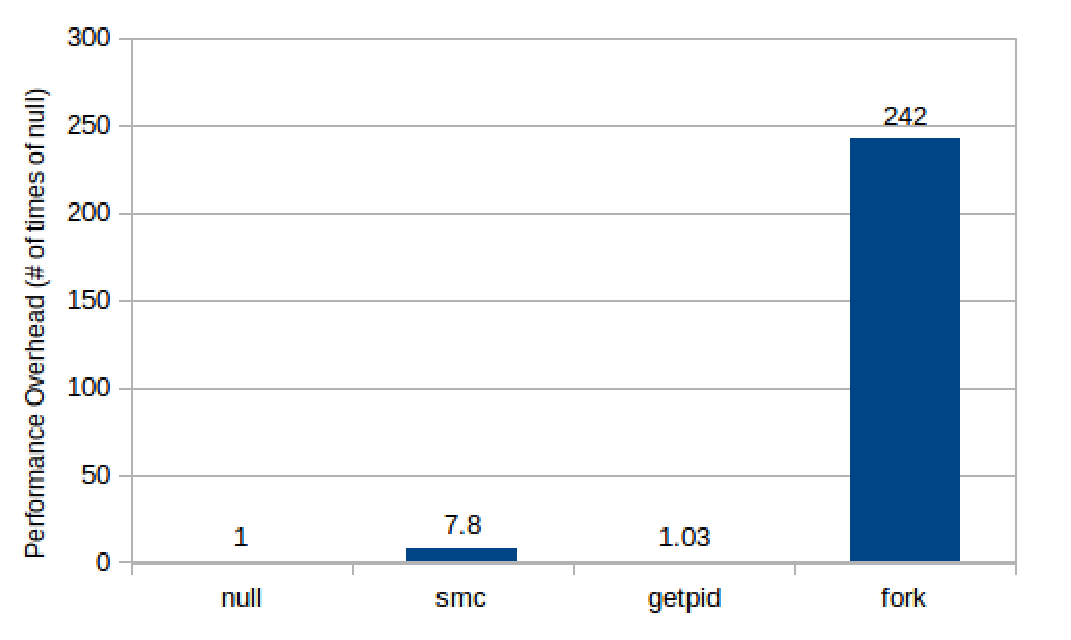
\includegraphics[width=1.0\columnwidth]{figures/syscall.eps}
	\caption{Performance Overhead Comparison of System Calls}
	\label{fig:syscall}
\end{figure}

\section{Discussion}
\label{sec:discussion}

As the world switch is primarily triggered by SMC instruction, the
super-privileged attacker in legacy OS can just block the call of SMC
instruction to mount the deny-of-service attack to prevent the user from
switching to TrustFA Agent in secure world. A solution would be to add a special
button on the smartphone and set the corresponding interrupt as secure. Once the
button is pressed, secure kernel will be triggered immediately.

The attacker can also mount the man-in-the-middle (MIM) attack by executing a
counterfeit of TrustFA Agent in normal world. Instead of the real TrustFA
Agent, the user will interact with the counterfeit. As the counterfeit is not
able to retrieve $K_{private}$ in secure world, the photos not encrypted with
the private key cannot pass the verification of the remote server.

As mentioned in section \ref{sec:implementation}, many peripheral drivers are
going to be ported to the secure kernel, which will increase the TCB size.
TrustFA is orthogonal to TrustUI \cite{TrustUI} minimizing the TCB in secure
world by placing only the driver's wrapper in secure world.

\section{Related Work}
\label{sec:related}

\noindent
{\bf Biometric Authentication~} 
Many biometric authentication techniques are involved in our life.
Fingerprint-based authentication is introduced with Apple's iPhone
\cite{iphone}. Karthikeyan \etal \cite{cmu-finger} compare the usability of
Apple’s iPhone 5S Touch ID fingerprint-based authentication with PIN-based
authentication and concludes that the former is better than the latter from
usability standpoint. In addition, face unlock is also implemented on Android
\cite{face-unlock}.  A fundamental limitation of biometric authentication is
that it is not very difficult for attacker to covertly obtain a person's photo
and video from social networks, or fingerprint pattern from an object or surface
touched by a person.  Researchers have developed numerous facial liveness
detection techniques \cite{Jain-MSU}, e.g., to capture spontaneous eye blinks or
lip movements \cite{Pan-ICCV}.  While it is useful for photo attacks, it cannot
deal with recorded videos.  3D face recognition has been widely studied in the
recent years \cite{Wang-PAMI, Amberg-FG, Chaua-3D}.  The 3D capturing process is
much more time consuming than 2D methods or entering a password.  Chen \etal
\cite{Chen-Sensor} make the first effort to employ motion sensors of smartphones
to improve the performance and security of facial authentication.  Our work also
utilize smartphone accelerometer to correlate 2D photo with 3D facial model and
leverage the Nose Angle Detection algorithm in \cite{Chen-Sensor}.  Regarding
Phase 2, our work assume a stronger threat model than \cite{Chen-Sensor}. While
\cite{Chen-Sensor} assumes the legacy OS is trusted, we assume it is potentially
malicious. In addition, the computation overhead of virtual camera attack
detection of \cite{Chen-Sensor} in Phase 2 is relatively high. By leveraging TrustZone, the overhead
of machine learning related computing can be eliminated and user only needs to
pay for the overhead of TrustZone world switch, which is in the magnitude of microsecond. 


\noindent
{\bf ARM TrustZone~}
TrustZone is the security extension of ARM. One of its application is to
protect the integrity of the OS kernel. TrustDump \cite{TrustDump} is a
TrustZone-based memory acquisition mechanism to reliably obtain the RAM memory
and CPU registers of the mobile OS kernel even if the OS has crashed or has
been compromised.  TZ-RKP \cite{TZ-RKP} and SPROBES \cite{SPROBES} propose
real-time OS protection mechanisms where the kernel is instrumented and all
critical kernel modifications will be trapped to TrustZone secure world.
Besides, TrustZone has been used to protect sensitive data.  DroidVault
\cite{DroidVault} establishes a secure channel between data owners and data
users while allowing data owners to enforce strong control over the sensitive
data with a minimal TCB in TrustZone secure world. TrustUI \cite{TrustUI}
proposes a new trusted path design for mobile devices that enables secure
interaction between end users and services based on ARM's TrustZone technology,
which is orthogonal to our work.  TLR \cite{TLR} enables the separation of
application security-sensitive logic from the rest of the application, and
isolates it from the OS and other apps. VeriUI \cite{VeriUI} introduces a TrustZone-assisted
credential-based authentication.  Unlike \cite{TrustUI}, our TrustFA is a
TrustZone-assisted facial authentication and we leverage the accelerometer to
different 2D counterfeit from 3D face.  Considering the urge requirement of
trusted reading from sensors such as GPS, camera, or microphones, Liu \etal
\cite{TrustSensor} implement a software abstraction for trusted sensors. In
our prototype, we will just implement our own software interfaces.

\section{Conclusion}
\label{sec:conclusion}

The facial authentication data flow on the smartphone can be divided into three
phases. TrustFA is the first effort that all three phases are secured.
Compared to prior works, the threat model regarding smartphone facial
authentication assumed in this paper is the most strongest. We leverage
TrustZone to guarantee the trust and freshness of data from camera and
accelerometer. In the future, people only need to focus on the first phase,
that is, how to more efficiently differentiate 2D flat photo from 3D user.


{\footnotesize \bibliographystyle{acm}
\bibliography{refs}}


%\theendnotes

\end{document}







